\documentclass[UTF8,a4paper,12pt]{ctexbook} 

 \usepackage{graphicx}%学习插入图
 \usepackage{verbatim}%学习注释多行
 \usepackage{booktabs}%表格
 \usepackage{geometry}%图片
 \usepackage{amsmath}
 \usepackage{amssymb}
 \usepackage{listings}%代码
 \usepackage{xcolor}  %颜色
 \usepackage{enumitem}%列表格式
 \usepackage{tcolorbox}
 \usepackage{algorithm}  %format of the algorithm
 \usepackage{algorithmic}%format of the algorithm
 \usepackage{multirow}   %multirow for format of table
 \usepackage{longtable} 
 \usepackage{tabularx} 	%表格排版格式控制
 \usepackage{array}	%表格排版格式控制
 \usepackage{hyperref} %超链接 \url{URL}
 % \setCJKmainfont{方正兰亭黑简体}  %中文字体设置
 % \setCJKsansfont{华康少女字体} %设置中文字体
 % \setCJKmonofont{华康少女字体} %设置中文字体

 \CTEXsetup[format+={\flushleft}]{section}

 \geometry{left=1.6cm,right=1.8cm,top=2cm,bottom=1.7cm} %设置文章宽度
 %%%% 设置图片目录
 \graphicspath{{figure/}}
 
 
 \pagestyle{plain} 		  %设置页面布局

 %代码效果定义
 \definecolor{mygreen}{rgb}{0,0.6,0}
 \definecolor{mygray}{rgb}{0.5,0.5,0.5}
 \definecolor{mymauve}{rgb}{0.58,0,0.82}
 \lstset{ %
 	backgroundcolor=\color{white},   % choose the background color
 	basicstyle=\footnotesize\ttfamily,      % size of fonts used for the code
 	%stringstyle=\color{codepurple},
 	%basicstyle=\footnotesize,
 	%breakatwhitespace=false,         
 	%breaklines=true,                 
 	%captionpos=b,                    
 	%keepspaces=true,                 
 	%numbers=left,                    
 	%numbersep=5pt,                  
 	%showspaces=false,                
 	%showstringspaces=false,
 	%showtabs=false,        
 	columns=fullflexible,
 	breaklines=true,                 % automatic line breaking only at whitespace
 	captionpos=b,                    % sets the caption-position to bottom
 	tabsize=4,
 	commentstyle=\color{mygreen},    % comment style
 	escapeinside={\%*}{*)},          % if you want to add LaTeX within your code
 	keywordstyle=\color{blue},       % keyword style
 	xleftmargin=.06\textwidth, 
 	stringstyle=\color{mymauve}\ttfamily,     % string literal style
 	frame=L,
 	rulesepcolor=\color{red!20!green!20!blue!20},
 	% identifierstyle=\color{red},
 	language=c++,
 }
 \author{\kaishu 郑华}
 \title{\heiti MySQL 数据库学习笔记}
 
\begin{document}          %正文排版开始
 	\maketitle
 \chapter{基础概念}
	 \section{术语}
		 \begin{itemize}
		 	\item  \textbf{数据库}: 数据库是一些关联表的集合。.
		 	\item  \textbf{数据表}: 表是数据的矩阵。在一个数据库中的表看起来像一个简单的电子表格。
		 	\item  \textbf{列}: 一列(数据元素) 包含了相同的数据, 例如邮政编码的数据。
		 	\item  \textbf{行}:一行(=元组,或记录)是一组相关的数据,例如一条用户订阅的数据。
		 	\item  \textbf{冗余}:存储两倍数据,冗余降低了性能,但提高了数据的安全性。
		 	\item  \textbf{主键}:主键是唯一的。一个数据表中只能包含一个主键。你可以使用主键来查询数据。
		 	\item  \textbf{外键}:外键用于关联两个表。
		 	\item  \textbf{复合键}:复合键(组合键)将多个列作为一个索引键,一般用于复合索引。
		 	\item  \textbf{索引}:使用索引可快速访问数据库表中的特定信息。索引是对数据库表中一列或多列的值进行排序的一种结构。类似于书籍的目录。
		 	\item  \textbf{参照完整性}: 参照的完整性要求关系中不允许引用不存在的实体。与实体完整性是关系模型必须满足的完整性约束条件,目的是保证数据的一致性。
		 \end{itemize}
		
	 
	 \section{教程集合地址}
	 	\url{https://blog.csdn.net/orangleliu/article/details/54694272}
	 	
\chapter{数据库基本操作}
	\section{SQL 分类}
		\begin{itemize}
			\item 数据库查询:代表关键字 \verb|select|
			\item 数据库操纵:代表关键字 \verb|insert delete update|
			\item 数据库定义:代表关键字 \verb|create drop alter|
			\item 事务控制:代表关键字 \verb|commit rollback|
			\item 权限控制:代表关键字 \verb|grant revoke|
		\end{itemize} 
	
	\section{常用命令}
		\begin{table}[H]
			\centering
			\caption{常用命令}
			\begin{tabular}{p{4cm}<{\centering}|p{11cm}<{\centering}}
				\hline
					类型  & 命令 \\
				\hline
					显示当前的数据库们  & \verb|show databases;| \\
					使用某个数据库	& 	\verb|use databaseName;| \\
					显示数据库中的表们	& \verb|show tables;|	\\
					查看表的创建语句	& \verb|show create table tableName;|	\\
					查看表的结构	& \verb|desc tableName;|	\\
					重名命(列名、表明)	& \verb|as| ,如 \verb|select lower(ename) as E from emp;|	\\
					创建数据库	& \verb|create database Name;|	\\
					设置字符集	& \verb|set NAMES 'utf8';| \verb|SET character_set_xx = utf8;|	\\
					终止一条语句	& \verb|\c|	\\
				\hline
			\end{tabular}
		\end{table}


\chapter{查询}
	\section{基本查询语句}
		\subsection{条件查询}
				\begin{table}[H]
					\centering
					\caption{查询符号}
					\begin{longtable}{c|m{10cm}}
						\hline
						运算符   &   功能说明\\
						\hline
						\verb|=| &  等于 \\
						\verb|!=| & 不等于 \\
						\verb|between ... and ..| & 等同于 \verb|>= ... and <= ...| \\
						\verb|is null| & 为\verb|null(is not null 不为空)| \\
						\verb|and| & 并且 \\
						\verb|or| & 或者\\
						\verb|in| & 包含,相当于多个\verb|or|,(not in 不在这个范围内)\\
						\verb|not| & 取非\\
						\verb|like| & 为模糊查询,支持\verb|%|或\verb|_|匹配,其中\verb|%|匹配任意个字符,\verb|_|只匹配一个字符\\
						\hline	
					\end{longtable}
				\end{table}
				
		\verb|example ->| 
			\begin{lstlisting}
// 执行顺序
	select  // 3
		xx, xx2, xx3
	 from   // 1
		XX
	 where  // 2
		 xx = xx;
		 
// in 示例	查找job是什么的,不是什么的	 
	select 
		ename,job
	from
		emp
	where
		job in('MANAGER','SALESMAN');
		
	select 
		ename,job
	from
		emp
	where
		job not in('MANAGER','SALESMAN');

// like 示例, 查找以S 开头的名字
	select 
		ename
	from 
		emp
	where
		ename like 'S%'	
			\end{lstlisting}
			
		\subsection{排序}
			\verb|order  by|
		
			\begin{lstlisting}
// order  示例 默认升序,(desc 降序)
select 
	ename,salary
from
	emp
order by
	salary

// 按照第几个字段排序	
select 
	ename,salary // 1,2 字段
from
	emp
order by
	2  // 第2个字段
	
// 多个字段排序, ename 升序,salary 降序,使用逗号分割
select 
	ename,salary
from
	emp
order by
	salary desc, ename
			\end{lstlisting}
		
		
		\subsection{数据处理函数(单行)}处理单行后结束
			\begin{itemize}[itemindent = 2em]
				\item \verb|lower| :转换小写
				\item \verb|upper| :转换大写
				\item \verb|substr| :取子串(被截取的串,起始位置,截取长度)
				\item \verb|length| :取长度
				\item \verb|trim| :去空格
				\item \verb|round| :四舍五入
				\item \verb|rand()| :生成随机数
				\item \verb|ifnull(xx, num)|: 可以将\verb|null| 值转换成一个具体值
			\end{itemize}
		
		
		\subsection{分组函数、聚合函数(多行)}
		
			处理多行后结束,自动忽略空值
			
			\textbf{先分组,然后再执行分组函数}, 而where在分组函数之前执行,所以不能
			
			\verb|where| 中不能出现分组函数
			
			\begin{itemize}[itemindent = 2em]
				\item \verb|count |:取得记录数
				\item \verb|sum |:求和
				\item \verb|avg |:求平均
				\item \verb|max |:取最大值
				\item \verb|min |:取最小值
			\end{itemize}
			
			\verb|distinct 去重关键字 -> select distinct job from emp;|  只能出现在所有\textbf{字段}的最前面
			
			\verb|select count(distinct job) from emp;|
			
	\section{分组查询}
			\subparagraph{group by}: \textbf{通过哪个或哪些字段进行分组},使用后select 后只能跟参与分组的字段和分组函数。
			
				\verb|example->| 找出每个工作岗位的最高薪水【先按照工作岗位分组,使用max 函数求每一组的最高工资】
				
					\begin{lstlisting}
// 先按照job 分组,然后对每一组使用max(salary) 求最大值。					
	select 			//3
		max(salary)
	from			//2
		emp;
	group by		//1
		job;	
		
// 结合where 限定分组前条件,即分组前过滤
	select
		job, max(sal)
	from 
		emp
	where 
		job != 'MANAGER'
	group by
		job;
	
					\end{lstlisting}
			
				\verb|example->| 找出每个工作岗位的平均薪水,要求显示平均薪水大于1500
				 where  处理不了
				
			\subparagraph{having} 与where 都是为了完成数据的过滤, \verb|where| 和 \verb|having| 后面都是添加过滤条件,\textbf{where是 在group by 之前执行}, \textbf{而having 是在group  by  后执行}。
			
				\begin{lstlisting}
//上例子解法
select 
	job,avg(sal)
from 
	emp
group by
	job
having 
	avg(sal) >  1500;
 
				\end{lstlisting}
			
			
			\subsection{查询语句总结}
			
				\subparagraph{关键字顺序不能变}:
				
					\begin{lstlisting}
	select 
		...
	from
		...
	where
		...
	group by
		...
	having
		...
	order by
		...
					\end{lstlisting}
			
				\subparagraph{执行顺序}:
					\begin{enumerate}[itemindent = 2em]
						\item \verb|from| 从某张表中检索数据
						\item \verb|where| 经过某条件进行过滤
						\item \verb|group by| 然后分组
						\item \verb|having| 分组之后不满意再过滤
						\item \verb|select| 查询出来
						\item \verb|order by| 排序输出
					\end{enumerate}
		
\section{连接查询}
			查询的时候\textbf{只从一张表检索数据}称为单表查询
			
			在实际的开发中,数据并不是存储在一张表中的,是同时存储在多张表中,这些表和表之间存在关系,我们在检索的时候通常需要将多长表联合起来取得有效数据,这种\textbf{多表查询}被\textbf{称为连接查询}或者叫做跨表查询。
			
			连接查询根据连接方式可以分为如下方式:
				\begin{itemize}[itemindent = 2em]
					\item  内连接
						\begin{itemize}[itemindent = 3em]
							\item 等值连接
							\item 非等值连接
							\item 自连接
						\end{itemize}
						
					\item  外连接
						\begin{itemize}[itemindent = 3em]
							\item 左外连接
							\item 右外连接
						\end{itemize}
						
					\item  全连接【几乎不用】
				\end{itemize}
				
		\subsection{内连接}		
				查找两张表匹配的数据。
				
				A表和B表能够完全匹配的记录查询出来,被称为内连接。
				\begin{figure}[H]
					\centering
					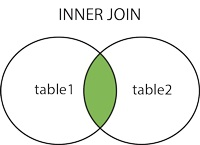
\includegraphics[scale=1]{innoJoin}
					\caption{内连接}
				\end{figure}
				
				\subparagraph{别名的使用,内连接的等值连接} 在进行多表连接查询的时候,尽量给表起别名,这样效率高,可读性高
					\begin{lstlisting}
// 将表emp 用别名 e表示..	

// 查询员工名与其对应的部门名
	select	
		e.ename, d.dname
	from 
		emp e, dept d;
	where 
		e.depno = d.depno
		
// SQL99 语法,使得表连接独立出来了,结构更清晰
	select 
		e.ename, d.dname
	from 
		emp e
	join	  // 内连接的inner 可以省略 
	    dept d
	on 
		e.depno = d.depno;
					\end{lstlisting}
					
				\subparagraph{内连接的非等值连接} 范围
					\begin{lstlisting}
// 找出员工名, 薪水,与其的薪水等级
	select 	
		e.name, e.sal, s.grade
	from
		emp e
	join 
		salgrade s
	on e.sal >= s.lower and e.sal <= s.higher;  // 可以使用between and 替代
					\end{lstlisting}
				 
				
				\subparagraph{内连接的自连接} 自己与自己连接,将自己视为两张表
					\begin{lstlisting}
//  找出每一个员工的上级领导,要求显示员工名以及对应的领导名
	表结构:
	empno ename mgr
	7369  SMITH 7123

// 要点:将自己视为两张表
	select
		a.ename empname, b.ename leaderName
	from 
		emp a
	join
		emp b
	on 
		a.mgr = b.empno;
					\end{lstlisting}	
				
	\subsection{外连接}

		A表和B表能够匹配的记录查询出来之外,\textbf{将其中一张表的记录}\textit{\underline{完全无条件}}的\textbf{完全查询出来},\textit{对方表没有匹配的记录,会自动模拟出NULL与之匹配}。
		
		$$\verb|外连接查询的结构条数| >= \verb|内连接的查询结果数量|$$
		
		可以添加除了内连接外的其他数据。
		\begin{figure}[H]
			\centering
			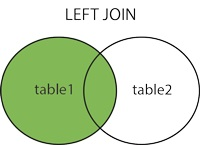
\includegraphics[scale=1]{leftjoin}
			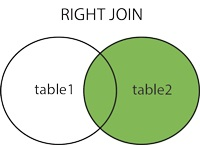
\includegraphics[scale=1]{rightjoin}
			\caption{外连接(左右)}
		\end{figure}
		
		
		\verb|example ->|找出每一个员工对应的部门名称,并且显示所有部门名称,注意部门可能没有员工。
		
				
		\subparagraph{左外连接}
			\verb|select e.ename, d.dname  from dept d left join emp e on e.deptno = d.deptno;|
		
		\subparagraph{右外连接}
			\verb|select e.ename, d.dname  from emp e right join dept d on e.deptno = d.deptno;|// outer  省略
				
		
		\subparagraph{总结}
			\textbf{希望将哪边表的数据完全显示出来},\verb| join| 的前边的修饰词 \verb|right left| 可以恰好说明,如上,\textbf{希望将dept表完全显示},那么\verb|先写dept| 的话,那么就在\verb|join 的左边|,就是 \verb|left join|.	
			
	
	\section{子查询}
		\url{https://www.cnblogs.com/zhuiluoyu/p/5822481.html}
	
	\section{union}
		UNION 操作符用于合并两个或多个 SELECT 语句的结果集
		
		\begin{lstlisting}
	SELECT column_name(s) FROM table_name1 // 如只有 1
	UNION
	SELECT column_name(s) FROM table_name2 // 如只有 2
	
	// 则结果为
	1
	2
		\end{lstlisting}	
		
		示例:\url{http://www.w3school.com.cn/sql/sql_union.asp}
			
	\section{limit}		
		用来获取一张表中的\textbf{某部分数据},只在MySQL数据特有的。
		\begin{lstlisting}
	// 找到员工表中前5条记录
	select ename 
	from emp 
	limit 5; //从下标0开始
	
	select ename
	from emp
	limit 0,5;// 从0下标开始,查找前5条
	
	// 找到工资在3到9名的员工
	select salary 
	form emp
	order by salary desc 
	limit 2,7;// 第三个的下标为2,一共7条
		\end{lstlisting}
	
	
	\section{执行顺序}
		\begin{lstlisting}
	FROM <left_table>
	ON <join_condition>
	<join_type> JOIN <right_table>
	WHERE <where_condition>
	GROUP BY <group_by_list>
	HAVING <having_condition>
	SELECT 
	DISTINCT <select_list>
	ORDER BY <order_by_condition>
	LIMIT <limit_number>
		\end{lstlisting}	
\chapter{增、删、改}
	\section{表、(with约束)}
		\subsection{create table tableName(columName type(length) [constraints]);}
			\begin{lstlisting}
	create table tableName(
		columnName dataType(length) constraints,
		...
	);
	set character_set_result = 'gbk';
	
	drop table tableName;
	drop table if exist tableName; //MySql 特色
	
	create table tableName as select * from existTableName; // 根据已创建的表创建新表
			\end{lstlisting}
		
		\subsection{数据类型}
			\begin{itemize}
				\item \verb|VARCHAR |可变长度字符串
				\item \verb|CHAR |定长字符串
				\item \verb|INT、BIGINT、FLOAT、DOUBLE | 基础数据类型
				\item \verb|DATE | 日期类型
				\item \verb|BLOB | 2进制大对象->图片
				\item \verb|CLOB | 字符大对象->比较大的字符串
			\end{itemize}
			
	\section{表结构}	
		\subsection{alter table tableName add newColumeName type(length);}
		
		\subsection{alter table tableName modify column newType(lenght);}
		
		\subsection{alter table tableName drop column;}
		
	\section{数据}
		\subsection{insert into tableName(column,..) values (value1,...);}
		
		\subsection{update tableName set columnName=newValue,... where xx;}
			当不指定条件时,将全表的该字段全部更新。
		
		\subsection{delete from tableName where xx;}
		
	\section{约束}
		\subsection{非空约束 not null}
			不能为空
			
		\subsection{唯一性约束 unique}
			不能重复但是可以为NULL,该字段值具有唯一性
			
			\paragraph{列级约束}
				\begin{lstlisting}
	create table tb(
	..,
	column varchar(32) unique,
	..);
				\end{lstlisting}
				
			\paragraph{表级约束}
				\begin{lstlisting}
	create table tb(
		...,
		column varchar(32),
		...,
		constraint consName unique(column1,...)
	);
				\end{lstlisting}
			
			当使用表级约束时,表示\textbf{多个字段联合}起来后唯一即可。而表级约束可以有名称是为了以后方便删除该约束。
			
		\subsection{主键约束 primary key}
			此列必须是\textbf{唯一并且非空}
			
			每个表都应该有一个主键,并且每个表只能有一个主键。但是注意,并不是说该主键只能在一列上作用,它具有表级约束的联合约束特性。
			\begin{lstlisting}
CREATE TABLE Persons
(
	P_Id int NOT NULL,
	LastName varchar(255) NOT NULL,
	FirstName varchar(255),
	Address varchar(255),
	City varchar(255),
	CONSTRAINT pk_PersonID PRIMARY KEY (P_Id,LastName)
)

			\end{lstlisting}
			在上面的实例中,只有一个主键 \verb|PRIMARY KEY(pk_PersonID),|然而,\verb|pk_PersonID| 的值是由两个列\verb|P_Id 和 LastName)|组成的。
			
		\subsection{外键约束 foreign key}
			\textbf{一个表中的} \verb|FOREIGN KEY| \textbf{指向另一个表中的} \verb|PRIMARY KEY|.
			
			\textbf{“Persons” 表}中的 \verb|“P_Id”| 列\textbf{是 “Persons” 表}中的 \verb|PRIMARY KEY|。
			
			\textbf{“Orders” 表}中的 \verb|“P_Id” |列\textbf{是 “Orders” 表}中的 \verb|FOREIGN KEY|。
			
			\verb|FOREIGN KEY| 约束用于\textbf{预防破坏表之间连接的行为}。
			
			\verb|FOREIGN KEY| 约束也能\textbf{防止非法数据插入外键列},\textit{因为它必须是它指向的那个表中的值之一}。
			
			\begin{lstlisting}
CREATE TABLE Orders
(
	O_Id int NOT NULL,
	OrderNo int NOT NULL,
	P_Id int,
	PRIMARY KEY (O_Id),
	FOREIGN KEY (P_Id) REFERENCES Persons(P_Id)
)
			\end{lstlisting}


\chapter{索引-重要}
	\section{简介}
		索引用于快速找出在某个列中有一特定值的行,不使用索引,MySQL必须从第一条记录开始读完整个表,直到找出相关的行,表越大,查询数据所花费的时间就越多,如果表中查询的列有一个索引,MySQL能够快速到达一个位置去搜索数据文件,而不必查看所有数据,那么将会节省很大一部分时间。

		\textbf{例如}:\textit{有一张person表,其中有2W条记录,记录着2W个人的信息。有一个Phone的字段记录每个人的电话号码,现在想要查询出电话号码为xxxx的人的信息}。
			\begin{itemize}
				\item \textbf{如果没有索引},那么将从表中第一条记录一条条往下\textbf{遍历},直到找到该条信息为止。
				\item \textbf{如果有了索引},那么会将\textbf{该Phone字段},\textbf{通过一定的方法进行存储},\textit{好让查询该字段上的信息时,能够快速找到对应的数据},而不必在遍历2W条数据了。其中MySQL中的索引的存储类型有两种:\verb|BTREE|、\verb|HASH|。
			\end{itemize}

	\section{优点、缺点和使用原则}
		\subparagraph{优点}
			\begin{itemize}[itemindent = 2em]
				\item 所有的MySql\textbf{列类型}(字段类型)\textbf{都可以被索引},也就是\textit{可以给任意字段设置索引}
				\item 大大加快数据的查询速度
			\end{itemize}
			
		\subparagraph{缺点}
			\begin{itemize}[itemindent = 2em]
				\item 创建索引和维护索引要耗费时间,并且随着数据量的增加所耗费的时间也会增加
				\item 索引也需要占空间
				\item 当对表中的数据进行增加、删除、修改时,索引也需要动态的维护,降低了数据的维护速度。
			\end{itemize}
			
		\subparagraph{使用原则}
			通过上面说的优点和缺点,我们应该可以知道,并不是每个字段度设置索引就好,也不是索引越多越好,而是需要自己合理的使用。
			\begin{itemize}[itemindent = 2em]
				\item \textbf{对经常更新的表}就\textit{避免对其进行过多的索引},对经常用于查询的字段应该创建索引
				\item \textbf{数据量小的表最好不要使用索引},因为由于数据较少,可能查询全部数据花费的时间比遍历索引的时间还要短,索引就可能不会产生优化效果
				\item \textbf{在一同值少的列上(字段上)不要建立索引},比如\textit{在学生表的"性别"字段上只有男,女两个不同值}。相反的,在一个字段上不同值较多可是建立索引
			\end{itemize}
			
	\section{索引的分类}
		\subparagraph{存储引擎支持类型}
			索引是在存储引擎中实现的,也就是说不同的存储引擎,会使用不同的索引
			\begin{itemize}[itemindent = 2em]
				\item \verb|MyISAM和InnoDB|存储引擎:\textbf{只支持BTREE索引}
				\item \verb|MEMORY/HEAP|存储引擎:\textbf{支持HASH和BTREE索引}
			\end{itemize}
			
		\subparagraph{单列索引}
			一个索引只包含单个列,但一个表中可以有多个单列索引。主要包括以下几种类型:
			\begin{enumerate}[itemindent = 2em]
				\item 普通索引:基本索引类型,没有什么限制,允许在定义索引的列中插入重复值和空值
				\item 唯一索引:索引列中的值必须是唯一的,但是允许为空值
				\item 主键索引:是一种特殊的唯一索引,不允许有空值。
			\end{enumerate}
			
		\subparagraph{组合索引}
			在表中的多个字段组合上创建的索引,\textbf{只有}在查询条件中\textit{使用了}\textbf{这些字段的左边字段时},索引才会被使用,使用组合索引时遵循最\textbf{左前缀集合}。
		
			\textbf{联合索引左侧字段用了范围查询,则其他字段无法用上}。
			
	\section{创建表添加索引}
		\subparagraph{创建普通索引}
			\begin{lstlisting}
// 方式一
CREATE TABLE book (
bookid INT NOT NULL,               
bookname VARCHAR(255) NOT NULL,           
authors VARCHAR(255) NOT NULL,            
info VARCHAR(255) NULL,                
comment VARCHAR(255) NULL,             
year_publication YEAR NOT NULL,           
INDEX(year_publication)               
);

// 方式二
CREATE TABLE book (
bookid INT NOT NULL,               
bookname VARCHAR(255) NOT NULL,           
authors VARCHAR(255) NOT NULL,            
info VARCHAR(255) NULL,                
comment VARCHAR(255) NULL,             
year_publication YEAR NOT NULL,           
KEY(year_publication)               
);                                                
			\end{lstlisting}
		\subparagraph{创建唯一索引}
			\begin{lstlisting}
CREATE TABLE t1
(
id INT NOT NULL,
name CHAR(30) NOT NULL,
UNIQUE INDEX UniqIdx(id)
); 
			\end{lstlisting}
		\subparagraph{创建主键索引}
			\begin{lstlisting}
CREATE TABLE t2
(
	id INT NOT NULL,
	name CHAR(10),
	PRIMARY KEY(id)
);
			\end{lstlisting}
		
		\subparagraph{创建组合索引}
			\begin{lstlisting}
CREATE TABLE t3
(
	id INT NOT NULL,
	name CHAR(30) NOT NULL,
	age INT NOT NULL,
	info VARCHAR(255),
	INDEX MultiIdx(id,name,age)
);
			\end{lstlisting}
			
			\textbf{组合索引就是遵从了最左前缀},\textit{利用索引中最左边的列集来匹配行,这样的列集称为最左前缀},例如,这里由id、name和age3个字段构成的索引,索引行中就按\verb|id/name/age|的顺序存放,\textbf{索引可以索引下面字段组合}\verb|(id,name,age)|、\verb|(id,name)|或者\verb|(id)|。如果要查询的字段不构成索引最左面的前缀,那么就不会是用索引,比如,age或者\verb|(name,age)|组合\textbf{就不会使用索引查询}
			
	
	\section{在已经存在的表上创建索引}
	
		\verb@ALTER TABLE 表名 ADD[UNIQUE|FULLTEXT|SPATIAL] [INDEX|KEY] [索引名](字段名)[ASC|DESC]@
		
		\verb@CREATE [UNIQUE|FULLTEXT|SPATIAL] [INDEX|KEY] 索引名称 ON 表名(字段名[length])[ASC|DESC]@
		
		\begin{itemize}
			\item ALTER TABLE book ADD INDEX BkNameIdx(bookname(30));
			\item CREATE INDEX BkBookNameIdx ON book(bookname);
		\end{itemize}
	
	\section{删除索引}
		\begin{itemize}
			\item ALTER TABLE 表名 DROP INDEX 索引名;
			\item DROP INDEX 索引名 ON 表名;
		\end{itemize}
	
	\section{索引背后的算法原理}
		\url{http://blog.codinglabs.org/articles/theory-of-mysql-index.html}	
	
	
	\section{索引设计概要}
		\url{https://draveness.me/sql-index-intro}
			
	\section{参考}
		\url{https://www.cnblogs.com/whgk/p/6179612.html}
			
	
	
\chapter{事务}

	
\chapter{进阶操作} 
	\section{binlog 日志-重要}
		\url{http://www.cnblogs.com/martinzhang/p/3454358.html}
		
		\subsection{GTID}
		
	\section{备份-重要}
		\begin{itemize}
			\item mysqldump: 逻辑备份; 单线程导入导出; 注意设定字符集; 
			\item mydumper: 逻辑备份; “多线程”导入导出; 无需关心字符集;
			\item innobackup/mysqlbackup: 物理备份; 速度较快;
		\end{itemize}
		\subsection{普通数据库备份}
			\verb|mysqldump -u root -p password --default-character-set=utf-8 dataname > dataname.sql|
			
			\verb|mysql -u root -p password --default-character-set=utf-8 dataname < dataname.sql|
		\subsection{备份到压缩文件}
			\verb@mysqldump -u root -p database | gzip > database.sql.gz@
			
			\verb@gzip < database.sql.gz | mysql -u root -p database@
		\subsection{增量备份}
			\verb@mysqlbinlog bin-log.000002 |mysql -uroot -ppassword@
		
	\section{InnoDB存储引擎}
	
	\section{视图}

	\section{主从模式-replication}
	
	\section{集群}
	
	\section{MySql 框架、执行流程}
		\url{https://www.cnblogs.com/annsshadow/p/5037667.html}
	
	\section{SQL语句优化}
		\subsection{explain 详解}
		
		
		\subsection{慢查询日志}
			MySQL \textbf{慢查询日志}是指 MySQL 中\textbf{执行时间超过} \verb|long_query_time| \textbf{阀值的 SQL 语句}。
			
			\verb|Dumbo| 默认每天零晨 \textbf{rotate 慢查询日志},按日期命名文件,每天一个文件,服务器上保留最近 8 天的慢查询日志文件。
			
			\textit{从慢查询日志中统计出执行比较频繁且执行时间比较久、扫描的行数也比较大的 SQL,可以针对这类 SQL 进行优化。}
		
			\paragraph{参数说明}
				慢查询日志相关的几个参数,有先后依赖关系,顺序如下:
				\begin{enumerate}[itemindent = 2em, itemsep = 0pt,partopsep=0pt]
					\item \verb|slow_query_log| \\ 是否启用慢查询日志功能,慢查询日志的内容可以在 \textbf{Dumbo 管理平台} \textit{实例管理 --> 日志管理 --> 慢查询日志} 上查看
					\item \verb|log_slow_admin_statements| \\ 是否记录administrative statements 语句到慢查询日志里。
					\item \verb|long_query_time| \\ 定义慢查询日志的触发条件,如果 SQL 实际执行时间(不包括锁的时间)超过 \verb|long_query_time| 定义的阀值,此 SQL 则被记录到慢查询日志里。
					\item \verb|min_examined_row_limit| \\ 只有慢查询语句的执行行数检查返回大于该参数指定值,此慢查询语句才被记录到慢查询日志中。
				\end{enumerate}
				
				\begin{table}[H]
					\centering
					\caption{慢查询日志参数}
					\begin{tabular}{p{6cm}<{\centering}|p{3cm}<{\centering}|p{3cm}<{\centering}|p{3cm}<{\centering}}
						\hline
							方法 &  MySQL默认值 &  Dumbo 默认值 & 能否自助修改\\
						\hline
						 \verb|slow_query_log| & OFF & ON &  否 \\
						 \verb|long_query_time| & 10s & 0.1s & 能 \\
						 \verb|log_slow_admin_statements| & OFF & ON & 否 \\
						 \verb|log_slow_slave_statements| & OFF & ON &否\\
						 \verb|min_examined_row_limit| & 0& 100 & 否 \\
						\hline
					\end{tabular}					
				\end{table}
				
				
				因此 \textbf{Dumbo 实例默认配置下},记录慢查询日志的条件是:
				\textbf{SQL 实际执行时间超过 0.1s,且此 SQL 的执行行数检查返回值大于 100}。
			\paragraph{优点}
				\begin{itemize}
					\item 语句调优 \\ 通过统计慢查询日志(可联系 Dumbo 值班),找出最耗时的 top 10 语句,优化完成后,再统计新的慢查询日志,一直重复,直到没有产生新的慢查询语句。
					\item 性能排查 \\ 如果一个实例的 CPU 使用率比较高,可以优先检查一下该实例的慢查询日志,如果慢查询日志刷得比较厉害,可以初步确认是由于 SQL 语句不够优化导致实例 CPU 使用率高,可以通过优化 SQL 来解决。
				\end{itemize}

		\subsection{查询优化-海量数据}
		
		\subsection{经验Tips}
			\url{https://coolshell.cn/articles/1846.html}
			
			\begin{enumerate}
				\item \textbf{EXPLAIN} \verb|SELECT| 查询 \\ 解释查询语句,查看是否使用到索引(\textbf{Key})
				\item 当只要一行数据时使用 \verb|LIMIT 1|  \\ 这样会在找到一条数据后停止搜索,而不是继续往后查少下一条符合记录的数据
				\item 为搜索字段建索引 \\ BTree Or Hash Better Than All
				\item 在Join表的时候使用相当类型的例,并将其索引
				\item 千万不要 \verb|ORDER BY RAND()|
				\item 避免 \verb|SELECT *|
				\item 永远为每张表设置一个ID
				\item 使用 \verb|ENUM| 而不是 \verb|VARCHAR|
				\item 尽可能的使用 \verb|NOT NULL|
				\item 无缓冲的查询
				\item 把IP地址存成 \verb|UNSIGNED INT|
				\item 固定长度的表会更快
				\item 垂直分割
				\item 拆分大的 DELETE 或 INSERT 语句
				\item 越小的列会越快
				\item 选择正确的存储引擎
			\end{enumerate}
		
		    
\end{document} 
 		    